\section{Formation Changes}
The proposed leader follower strategy is readily capable of providing manned leaders the ability to change formation types. This need is surprisingly great for SPT operations due to the temporal and spatial terrain variation. At certain points in the operating season and at different areas along the route, there is added benefit from tractors repeatedly compacting the same snow by driving in each other's tracks. From a modeling perspective, cold temperatures and compaction translate to changes in Bekker pressure-sinkage parameters but also to changes in cohesion. To achieve this compaction, drivers would use a column formation shown in Fig. \ref{fig:Leader_Follower_Formation_Column} where the lateral offset $D_{lat} = 0\hspace{1mm}m$. At later points in the operating season when temperatures are warmer or in softer parts, the tractors can create large ruts and destroy the flagged route especially with reptitive driving in the same tracks. Under these conditions, the staggered formation shown in Fig. \ref{fig:Leader_Follower_Formation_Staggered} is most appropriate. A close look at this diagram will show that the follower vehicle is avoiding driving in its leader's rut while not creating an unnecessary offset distance. This formation type is used for simulation results of the previous section. To adjust between these two formation types, the way point lateral offset from the tractor $D_{lat}$ can be gradually adjusted. Using this adjustment and the look-ahead approach for heading correction, stable transitions between formations will occur. It should be noted that if terrain conditions make it imperitive that the follower should drive in the tractor's rut or avoid it at all costs, small look-ahead distances $D_{LA}$ should be used so that way points are strictly followed.

The other formation adjustment to consider is the longitudinal offset specified by the parameter $D_{long}$. This could be done using techniques from trajectory optimization using a simple kinematic vehicle model, but a more simple technique is sufficient. In normal operation where a single formation is maintained, eq. \ref{eq:velocity_reference} provides the velocity reference to the controller. During a formation change, the proposed velocity reference given to the follower is
\begin{equation}
    v_{ref} = C + v_{leader}
\end{equation}
where $C$ is a low valued constant between -1 and 1 $m/s$ to be determined. This could be based on the current engine percent load conditions of the leader or a fixed value determined ahead of time.
\begin{figure}[hb]
\begin{subfigure}{1\textwidth}
\centering
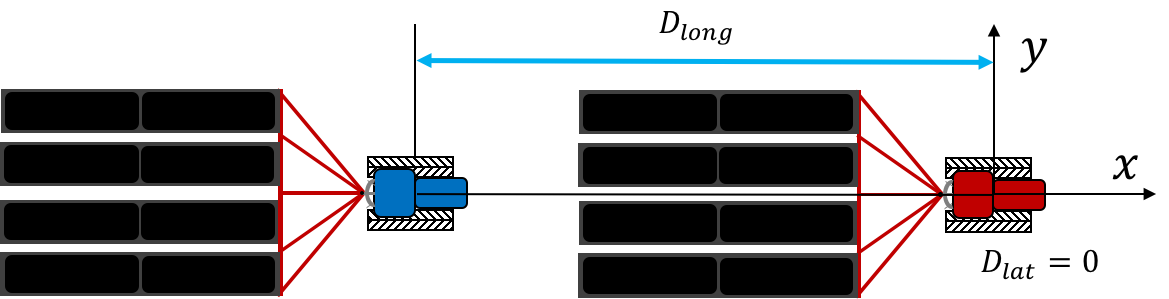
\includegraphics[height = 2.75 cm, keepaspectratio]{Leader_Follower_Formation_Column}
\caption{}
\label{fig:Leader_Follower_Formation_Column}
\end{subfigure}
\begin{subfigure}{1\textwidth}
\centering
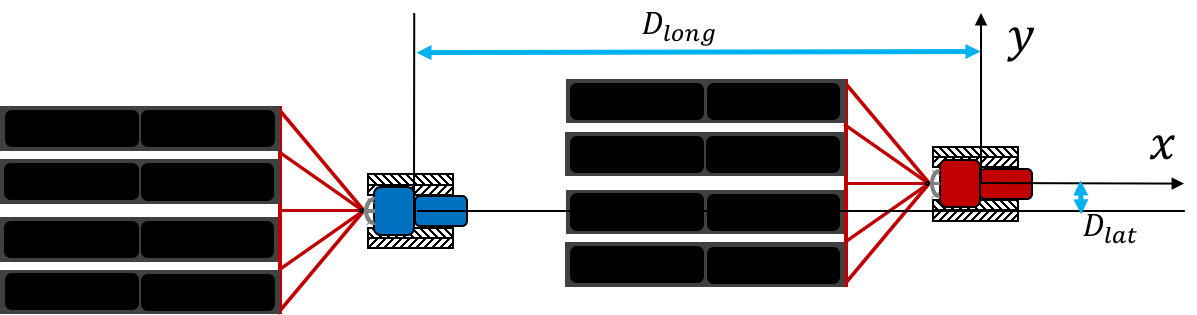
\includegraphics[height = 2.87cm, keepaspectratio]{Leader_Follower_Formation_Staggered}
\caption{}
\label{fig:Leader_Follower_Formation_Staggered}
\end{subfigure}
\caption{(a) Column leader follower formation  (b) Staggered leader follower formation  (a \& b) Leader tractors are colored red, follower tractors are colored blue.}
\label{fig:Leader_Follower_Concept}
\end{figure}